\begin{song}{title=\centering Pyšný Janek \\\normalsize Jaromír Nohavica  \vspace*{-0.3cm}}  %% sem se napíše jméno songu a autor
\moveright \stred \vbox{      %Varianta č. 1  ---> Jeden sloupec zarovnaný na střed	

\sloka 
	/: ^{A}Pyšný Janku na okénku,

	pyšný v poli,Dpyšný v ^{A}šenku. :/
	
	/:^{E}Kajže ty si ^{F#mi}najdeš ^{D\,A}ženku. :/
	
	/:^{E}Kajže ty si ^{F#mi}najdeš ^{D\,A}ženku, :/, jé.

\sloka
	/: Děvuchy do kola chodí,

	za ruky se spolu vodí. :/
	
	/: Ani jedna neuškodí. :/
	
	/: Ani jedna neuškodí, :/ jé

\sloka
	/: Bo ty, švarný, pyšný Janku,
	
	nechceš žádnů za galánku. :/
	
	/: Inum koňa, inum šklanku. :/

	/: Inum koňa, inum šklanku, :/ jé.


}
\setcounter{Slokočet}{0}
\end{song}


\begin{figure}[h]
\centering
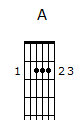
\includegraphics[scale=1.5]{../Akordy/a.png}
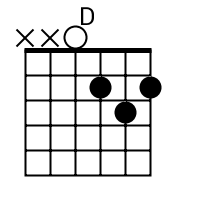
\includegraphics[scale=1.5]{../Akordy/d.png}
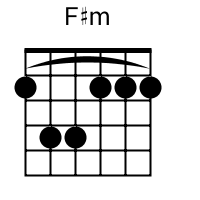
\includegraphics[scale=1.5]{../Akordy/fxm.png}
\end{figure}
